	\marginnote{
	\begin{minipage}{5.5cm}
		\begin{figure}[H]\centering
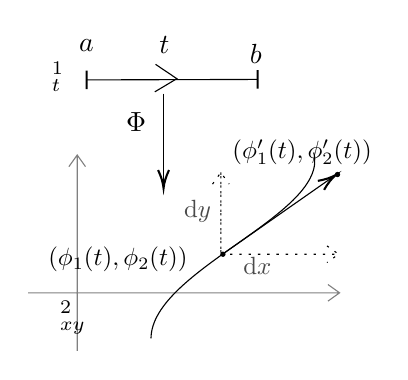
\begin{tikzpicture}[x=0.6pt,y=0.6pt,yscale=-1,xscale=1]
%Shape: Axis 2D [id:dp41021135976261514] 
\draw [color={rgb, 255:red, 128; green, 128; blue, 128 }  ,draw opacity=1 ] (5,256) -- (192.5,256)(34.5,173) -- (34.5,291) (185.5,251) -- (192.5,256) -- (185.5,261) (29.5,180) -- (34.5,173) -- (39.5,180)  ;
%Straight Lines [id:da5315594181633504] 
\draw    (143.15,127.48) -- (40.14,127.77) ;
\draw [shift={(40.14,127.77)}, rotate = 359.83000000000004] [color={rgb, 255:red, 0; green, 0; blue, 0 }  ][line width=0.75]    (0,5.59) -- (0,-5.59)   ;
\draw [shift={(143.15,127.48)}, rotate = 359.83000000000004] [color={rgb, 255:red, 0; green, 0; blue, 0 }  ][line width=0.75]    (0,5.59) -- (0,-5.59)   ;
\draw   (81.67,118.39) -- (94.51,127.04) -- (81.22,134.97) ;

%Shape: Circle [id:dp36661837654320517] 
\draw  [fill={rgb, 255:red, 0; green, 0; blue, 0 }  ,fill opacity=1 ] (123.5,232.75) .. controls (123.5,232.06) and (122.94,231.5) .. (122.25,231.5) .. controls (121.56,231.5) and (121,232.06) .. (121,232.75) .. controls (121,233.44) and (121.56,234) .. (122.25,234) .. controls (122.94,234) and (123.5,233.44) .. (123.5,232.75) -- cycle ;
%Shape: Circle [id:dp3341593596220296] 
\draw  [fill={rgb, 255:red, 0; green, 0; blue, 0 }  ,fill opacity=1 ] (192.5,184.75) .. controls (192.5,184.06) and (191.94,183.5) .. (191.25,183.5) .. controls (190.56,183.5) and (190,184.06) .. (190,184.75) .. controls (190,185.44) and (190.56,186) .. (191.25,186) .. controls (191.94,186) and (192.5,185.44) .. (192.5,184.75) -- cycle ;
%Shape: Axis 2D [id:dp8708604035951039] 
\draw [dash pattern={on 0.84pt off 2.51pt}] (121,232.75) -- (191.93,232.75)(121,183.53) -- (121,232.75) -- cycle (184.93,227.75) -- (191.93,232.75) -- (184.93,237.75) (116,190.53) -- (121,183.53) -- (126,190.53)  ;
%Straight Lines [id:da5074920899678971] 
\draw    (122,232.75) -- (188.61,186.15) ;
\draw [shift={(190.25,185)}, rotate = 505.02] [color={rgb, 255:red, 0; green, 0; blue, 0 }  ][line width=0.75]    (10.93,-3.29) .. controls (6.95,-1.4) and (3.31,-0.3) .. (0,0) .. controls (3.31,0.3) and (6.95,1.4) .. (10.93,3.29)   ;

%Curve Lines [id:da6202345516128739] 
\draw    (78.93,283.43) .. controls (79.37,241.87) and (186.93,208.53) .. (176.93,171.53) ;


%Straight Lines [id:da48049376839429636] 
\draw    (86.5,136) -- (86.5,191) ;
\draw [shift={(86.5,193)}, rotate = 270] [color={rgb, 255:red, 0; green, 0; blue, 0 }  ][line width=0.75]    (10.93,-3.29) .. controls (6.95,-1.4) and (3.31,-0.3) .. (0,0) .. controls (3.31,0.3) and (6.95,1.4) .. (10.93,3.29)   ;


% Text Node
\draw (40,107) node   {$a$};
% Text Node
\draw (142,112) node   {$b$};
% Text Node
\draw (87,107) node   {$t$};
% Text Node
\draw (70,153) node   {$\Phi $};
% Text Node
\draw (59,236) node [scale=0.9]  {$( \phi _{1}( t) ,\phi _{2}( t))$};
% Text Node
\draw (169.93,171.53) node [scale=0.9]  {$( \phi '_{1}( t) ,\phi '_{2}( t))$};
% Text Node
\draw (143,240) node [scale=0.9,color={rgb, 255:red, 74; green, 74; blue, 74 }  ,opacity=1 ]  {$\mathrm{d} x$};
% Text Node
\draw (107,207) node [scale=0.9,color={rgb, 255:red, 74; green, 74; blue, 74 }  ,opacity=1 ]  {$\mathrm{d} y$};
% Text Node
\draw (23,126) node   {$\R^{1}_{t}$};
% Text Node
\draw (32,271) node   {$\R^{2}_{xy}$};
\end{tikzpicture}
			\caption{Mapeo del caso 1-2.}\label{ch0d2}
		\end{figure}
\end{minipage}}[-4em]